Para definir el concepto de aprendizaje automático con una buena perspectiva, debemos, primeramente definir qué es la inteligencia artificial. 

La inteligencia artificial en un enfoque de actuar humano se define como ``El arte de crear máquinas que realicen funciones que requieren inteligencia cuando las realizan personas''.\cite[p. 2]{stuart2010artificial}. De esta rama de la informática han surgido campos que actualmente están siendo potencialmente estudiados como: el procesamiento del lenguaje natural, el aprendizaje automático, el aprendizaje profundo, la visión por computadora, etc.

Los avances en estas áreas de estudio han dado como resultado aplicaciones populares, tales como: modelos de clasificación de texto, modelos de traducción de idiomas, cualquier modelo generativo, sistemas de conducción autónomos de vehículos, etc.

Muchos de estos sistemas y aplicaciones inteligentes son parte de una vida diaria, donde probablemente se usen de manera desapercibida, se podría decir que ha surgido la nueva fiebre por la inteligencia artificial. Nunca antes como ahora la inteligencia artificial había sido tan nombrada en noticias, medios de comunicación o revistas científicas, y tan ampliamente usada por cualquiera que así lo necesite, tenga o no conocimiento técnico de esta rama de estudio. Una de las razones sobre la que descansa toda esta popularidad es el aprendizaje automático.

El aprendizaje automático se enfoca en la creación de algoritmos y modelos que permiten a las máquinas aprender patrones a partir de una gran cantidad de datos, capacitándolas para llevar a cabo tareas específicas sin necesidad de seguir instrucciones programadas.

Arthur Samuel, en 1959, definió el aprendizaje automático como: ``El campo de estudio que otorga a las computadoras la capacidad de aprender sin ser programadas explícitamente'' \cite[p. 281]{geron2019hands}.

Posteriormente, en 1997, Tom Mitchell proporcionó otra definición clave: ``Se dice que un programa de computadora aprende de la experiencia E con respecto a alguna tarea T y alguna medida de desempeño P, si su desempeño en T, medido por P, mejora con la experiencia E''\cite[p. 281]{geron2019hands}.

En el campo del aprendizaje automático, se encuentran algoritmos fundamentales que son comúnmente empleados en tareas relacionadas con texto, algunos de estos son: la regresión logística, los árboles de decisión y Naive Bayes. Estos algoritmos tienen notables limitaciones en cuanto a su capacidad para aprender representaciones jerárquicas de texto, captura de contexto, modelar relaciones no lineales y escalar eficazmente. Pero en casos donde el conjunto de datos es reducido y la tarea no implica complejidades profundas en el análisis de características del texto, estos modelos más simples pueden mostrar un rendimiento satisfactorio.

Ya que se menciona al conjunto de datos necesario para entrenar estos y otros algoritmos de aprendizaje es importante aclarar que uno de los desafíos del aprendizaje automático radica en la recopilación de datos. Lo ideal sería contar con miles de millones de datos que se encuentren balanceados, limpios, etiquetados y que además sean representantes valiosos para la tarea a realizar. Sin embargo esta situación es casi imposible de alcanzar. Encontrar conjuntos de datos más o menos adecuados para alguna tarea ya puede considerarse un éxito y un gran avance para el proyecto. Sin embargo, si no se obtiene siquiera esa ventaja, debe procederse a una exhaustiva recopilación de datos que además implica un riguroso proceso de revisión, limpieza, análisis, preprocesamiento, etiquetado y muchas otras tareas más.

\begin{figure}[h!]
	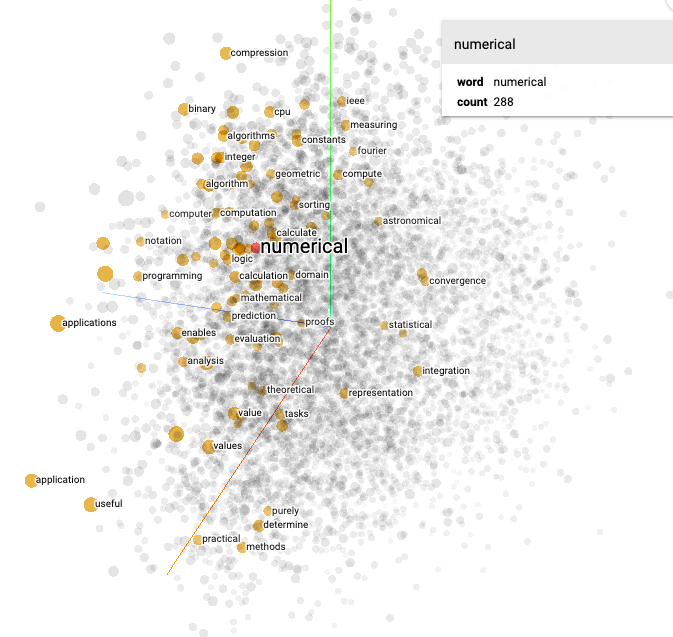
\includegraphics[width=0.65\textwidth]{capitulo2/figuras/an1.png}
	\caption{Representacion vectorial tridimensional
		\\\textit{Fuente: Elaboracion Propia}}
	\label{fig:tensorboard}
\end{figure}

Uno de los subcampos fundamentales del aprendizaje automático, que depende en gran medida de la calidad y cantidad de los datos, es el aprendizaje profundo. El aprendizaje profundo se centra en el entrenamiento de redes neuronales con múltiples capas apiladas, cada una compuesta por neuronas interconectadas que realizan operaciones matemáticas con los datos.

La diferencia principal entre las redes neuronales tradicionales y las redes neuronales profundas radica en la capacidad de estas últimas para comprender características complejas de los datos. Un ejemplo notable de esta capacidad se evidencia en modelos de aprendizaje profundo como Word2Vec, cuya función es representar palabras como vectores densos.\\
Word2Vec tiene en cuenta el contexto en el que aparecen las palabras, lo que facilita la captura de significados contextualmente relevantes. En la figura \ref{fig:tensorboard}  se puede observar una representación de embeddings de 10,000 palabras en la interfaz de Tensorflow. Con el vector de la palabra ``numerical'' como punto de referencia, se pueden observar los vectores de las palabras más cercanos a numerical que, resaltan ya sea por contexto, sintaxis o similitud semántica. El cálculo de estas características complejas sólo puede llevarse a cabo mediante redes de aprendizaje profundo. 

Esta breve introducción tiene como objetivo dar una perspectiva amplia sobre estos conceptos fundamentales con algunos ejemplos que permitan comprender las aplicaciones del aprendizaje automático y profundo. En las siguientes secciones del capítulo se realizará una exploración más profunda sobre el funcionamiento, las ventajas y limitaciones de estas dos áreas de estudio.


